\documentclass[11pt]{article}
\usepackage[letterpaper,margin=0.85in]{geometry}
\usepackage[T1]{fontenc}
\usepackage[utf8]{inputenc}
\usepackage{amsmath,amssymb,amsfonts,bm}
\usepackage[table]{xcolor}
\usepackage{graphicx}
\usepackage{booktabs}
\usepackage{array}
\usepackage{multirow}
\usepackage{caption}
\usepackage{subcaption}
\usepackage{cite}
\usepackage[article]{ragged2e}
\usepackage{parskip}
\usepackage{hyperref}

% initialize counters for reviewer number and comment number
\newcounter{reviewer}
\setcounter{reviewer}{0}
\newcounter{point}[reviewer]
\setcounter{point}{0}
\renewcommand{\thetable}{\Roman{table}}
\setcounter{table}{0}
\captionsetup[table]{skip=8pt}
% Set the format of reviewer comment numbers and responses.
% "Review 1.k" in this letter = tag "R1.k" in the revised manuscript.
\renewcommand{\thepoint}{Review\,\thereviewer.\arabic{point}}
\newcommand{\point}[1]{\refstepcounter{point}  \bigskip \hrule \medskip \noindent \textit{{\fontseries{b}\selectfont \thepoint } #1}\par}
\newcommand{\reply}{\medskip \noindent \textbf{Reply}:\ }

% Set the format for reviewer headings
\newcommand{\reviewersection}{\stepcounter{reviewer}
                  \section*{To Reviewer \#\thereviewer}}

% Set the format for reviewer headings
\newcommand{\editorsection}{\section*{To Associate Editor}}

% Revised manuscript material reproduced in this letter (red, as in the
% manuscript).
\newcommand{\revisedheading}[1]{\medskip\noindent\textbf{Revised material
  reproduced in full (#1):}\par}
\newenvironment{revised}{\par\color{red}}{\par}
% Location of a comment in the decision letter.
\newcommand{\loc}[1]{\textup{[#1]}}

%Table Space
\newcommand\T{\rule{0pt}{2.5ex}}       % Top strut
\newcommand\B{\rule[-1.3ex]{0pt}{0pt}} % Bottom strut


\hypersetup{
    colorlinks,
    linkcolor={blue!80!black},
    citecolor={blue!80!black},
    urlcolor={blue!80!black}
}


%%%%%%%%%%%%%%%%%%%%%%%%%%%%%%%%%%%%%%%%%%%%%%%%%%%%%%%%
\title{Proteomics-Integrated Digital Twin State Space for Dopaminergic Stem Cell Differentiation \\ (Manuscript Number: CMPB-D-26-05530)}
\author{}
\date{}
\begin{document}

\maketitle

\vspace{10 pt}

\newpage
\editorsection
\justifying
Thank you for the careful and constructive assessment of manuscript CMPB-D-26-05530. We have completed a major revision in response to every point raised by Reviewers~1 and~2. Each comment is reproduced verbatim below, followed by a direct response and the corresponding revised manuscript material. To make the response self-contained, we reproduce the relevant revised passages, tables, and figures here, so that the reviewers do not need to search the manuscript to verify what changed. In the revised manuscript, all material inserted or substantively rewritten is shown in \textcolor{red}{red}, and each change is preceded by a superscript tag naming the comment it answers. Language-only corrections from the full proofread are shown in red without a tag. Table~\ref{edited} summarises the principal changes.

 \begin{table}[!thbp]
    \caption{Summary of major differences between the submitted and revised manuscripts.}
    \label{edited}
    \centering
    \begin{tabular}{l|c|c}
    \hline\hline
    Manuscript element & Submitted & Revised\T\B\\ \hline\hline
        Number of Figures                      & 4 &  5 \T\B\\\hline
        Number of Tables                       & 8 & 10 \T\B\\\hline
        Supplementary Tables                   & 0 & 1 \T\B\\\hline
        Number of References                   & 26 & 26\textsuperscript{$*$} \T\B\\ \hline\hline
    \multicolumn{3}{l}{\footnotesize\textsuperscript{$*$}One added at Reviewer~1's request; one incorrect citation removed (correction~7 below).}
    \end{tabular}
    \vspace{-4mm}
    \end{table}

\medskip
The main changes are:
\begin{itemize}
  \item \textbf{Objectives and framing.} The Introduction now ends with an explicit objectives paragraph: the primary contribution is the proteomics-integrated state representation; stage separability (Task~A) and trajectory prediction (Task~B) are two distinct tests of it, reported in separate Results subsections; blockchain provenance is supporting infrastructure.
  \item \textbf{Proteomics transparency.} New text on proteomic processing (filtering, gene mapping, sample selection, missing values, replicate aggregation); a new subsection on the cross-dataset stage correspondence with a stage-mapping table (Table~2); a per-replicate table from sample label to model stage (Table~3); and a new figure of the individual replicates (Figure~2).
  \item \textbf{Trajectory construction and leakage.} An exact description of how the 200 trajectories were sampled and how $Pr$ is assigned to them (new Eq.~6), and a leakage-control paragraph.
  \item \textbf{Statistics.} Paired bootstrap 95\% confidence intervals for the Task~B MAE reduction (Table~7), an explicit statement of what the 20 seeds do and do not vary, and a justification of the paired Wilcoxon test.
  \item \textbf{Interpretation.} Task~A is presented as stage-separability evidence on the $Pr$ axis, not model superiority; the Task~B gain is attributed to the added $Pr$ dimension, with confidence intervals showing that the $P$ and $D$ errors are unchanged.
  \item \textbf{Discussion and limitations.} A new subsection summarising what each validation experiment establishes, shorter and plainer blockchain text, and seven numbered limitations (small replicate count, cross-study batch effects, no external validation, Task~A scope, marker coverage, phosphoproteomics, unvalidated drug screening).
  \item \textbf{Other.} Code and data availability statement; the requested citation; Figure~1 enlarged; blockchain deployment details moved to Supplementary Table~S1; the abstract rewritten.
\end{itemize}

\medskip
\noindent\textbf{Author corrections.} While answering the comments on reproducibility, we re-checked every methodological statement against the released code and corrected the following descriptions. None of these corrections changes any reported number; they make the text match what was actually run.
\begin{enumerate}
  \item The D11 proteomic score of each trajectory is drawn from a detection-floor distribution $\mathcal{N}(0, \sigma_{\text{D11}}/2)$, not from $\mathcal{N}(1.83, 3.17)$ as originally written. Two of the three iPSC replicates contain no marker, and the stage mean of 1.83 is produced by a single TH detection (Table~3, Figure~2). The rationale is given in Section~3.3 (Eq.~6).
  \item $P$ and $D$ are scaled with fixed bounds computed over all 161,584 cells, as in the published baseline; only $Pr$ uses training-split bounds. The original text stated that all three scores used training-split bounds. Section~3.3 now explains why the fixed, label-free bounds cannot leak label information.
  \item Eq.~9 (MAE) now divides by the number of state dimensions $k$, matching the implementation, which averages the error over dimensions.
  \item The Random Forest uses 200 trees for both tasks (the text said 100 for Task~A), and the linear model for Task~A is logistic regression (the Figure~1 caption said Ridge).
  \item D11 is the floor-plate progenitor stage of the transcriptomic dataset, not a pluripotent stage.
  \item Because $Pr$ is drawn independently of $P$ and $D$ within each stage, the near-zero within-stage correlations of Table~4 are expected by construction. We now present them as confirming that the assembled state introduces no spurious coupling, rather than as evidence of biological orthogonality, and we revised every statement that relied on them (contribution list, Sections~3.5.6, 4.2 and~4.3.1, and the Figure~4 caption).
  \item During proofreading we found two citation problems in Section~2. A review of digital twins in tumour therapy had been cited as one of ``the deepest publicly available iPSC-DA proteomes''; it has been removed from that sentence and from the reference list. The description of Tasaki et al.\ overstated their finding (``entirely absent from transcriptomic profiles''); it now says that protein-level changes are only partly predictable from mRNA.
  \item The one-sided Wilcoxon hypothesis in Section~3.5.3 is now written in terms of the MAE ($\text{MAE}_{3\text{D}} < \text{MAE}_{2\text{D}}$) rather than the state vectors, and the deterministic-ablation text now refers to the sampling distribution of Eq.~6.
\end{enumerate}

\newpage
\reviewersection

We thank the reviewer for the positive assessment of the objectives, methodology, statistical analysis, figures, and the combination of transcriptomic and proteomic information, and for the specific suggestions that helped us sharpen the framing and the interpretation. Every suggestion has been implemented.

\point{The authors may further clarify in the introduction whether the main contribution is the proteomics-integrated state-space construction, the improved trajectory prediction, or the blockchain-based reproducibility layer. This will make the novelty easier to follow for readers. / Please clarify whether the main novelty is the proteomics-integrated Pr-axis, the improved trajectory prediction, or the blockchain-based provenance layer.}

\reply{The main novelty is the proteomics-integrated state-space construction, i.e.\ the $Pr$ axis. Trajectory prediction is one of the two tests used to evaluate that representation, and the blockchain layer is a secondary, supporting contribution that does not affect any modelling result. We added an Objectives paragraph at the end of the Introduction that states this hierarchy, reordered the contribution list by importance with the main novelty and the supporting contribution labelled, and stated the objective in the abstract.}

\revisedheading{Introduction}
\begin{revised}
The primary objective of this study is the construction and validation of a proteomics-integrated state representation for iPSC-DA differentiation. Two questions are asked of this representation, and they are kept separate throughout the paper: \textit{(O1) stage separability} --- does the added proteomic axis distinguish the three differentiation stages that the transcriptomic axes confuse? (Task~A); and \textit{(O2) trajectory prediction} --- does the 3D state improve forecasting of the late-stage state from earlier states, and on which axes? (Task~B). O1 is a diagnostic of the representation rather than a predictive goal in itself; O2 is the forecasting question for which a digital twin is ultimately intended. The blockchain provenance layer is a secondary, supporting contribution that makes the multi-source pipeline verifiable; it does not affect any modelling result. In order of importance, the four contributions of this work are: [\ldots] (1) a proteomics-integrated 3D state space [\ldots] (the main novelty of the work); [\ldots] (4) a deployable DLT provenance layer [\ldots] (a supporting contribution).
\end{revised}

\revisedheading{Abstract, second sentence}
\begin{revised}
This study constructs and validates a proteomics-integrated state representation for dopaminergic differentiation of induced pluripotent stem cells (iPSC-DA).
\end{revised}

\point{The authors should slightly improve reproducibility by providing clearer details on how the 200 trajectories were sampled from the scRNA-seq dataset and how Pr values were assigned to individual trajectories.}

\reply{We now describe both steps exactly as implemented. Each trajectory pairs one cell drawn uniformly at random from each of the D11, D30, and D52 cell pools, independently of one another; because scRNA-seq is destructive, the three cells are different cells and a trajectory is a population-level pseudo-trajectory. The 200 trajectories are the published tensor of the baseline study and are identical in every run. $Pr$ is then assigned to each trajectory and stage by one random draw from the stage distribution estimated from the proteomic replicates (new Eq.~6). D11 is anchored at the detection floor, and we explain why. Both procedures are in Section~3.3, and the replicate data and sampling distributions are shown together in the new Figure~2 (reproduced under Review~2.11).}

\revisedheading{Section~3.3, Assigning $Pr$ to trajectories and Trajectory assembly}
\begin{revised}
\textbf{Assigning $Pr$ to trajectories.} Proteomics and scRNA-seq were measured on different cells, so no cell has a measured $Pr$ value. Each trajectory $i$ instead receives, at each stage $t$, one value drawn independently of its $P$ and $D$ values:
\begin{equation*}
  Pr^{(i)}_{t} \sim
  \begin{cases}
    \mathcal{N}\bigl(\mu_{t},\, \sigma_{t}\bigr), & t \in \{\text{D30}, \text{D52}\},\\[2pt]
    \mathcal{N}\bigl(0,\, \sigma_{\text{D11}}/2\bigr), & t = \text{D11},
  \end{cases}
  \qquad\text{(Eq.~6)}
\end{equation*}
with $(\mu_{t}, \sigma_{t})$ the replicate statistics above. D11 is anchored at the detection floor rather than at its replicate mean because two of the three iPSC replicates contain no $\mathcal{G}_{Pr}$ marker at all and the mean of 1.83 is produced by a single TH detection in one replicate (Table~3); a pre-DA stage is expected to sit at the floor of the DA-pathway axis. The floor keeps a small spread, half the D11 replicate standard deviation ($\sigma = 1.59$), so that D11 values are not all identical. This anchor was used for every result reported, and it replaces the description $\mathcal{N}(\mu_{\text{stage}}, \sigma_{\text{stage}})$ for all stages given in the original submission; it is shown alongside the replicate data in Figure~2, and because D11 ($\approx 0$) and D30 ($\approx 19$) are far apart on the $Pr$ axis under either choice, it does not affect the stage ordering that the analyses rely on. The random draws are made with the run's seed (Section~3.5.3). Within-stage sampling preserves a plausible within-stage spread; the deterministic ablation (Section~3.5.7), which sets every value to the stage centre, shows that this spread carries no additional signal.

[\ldots] Concretely, for each trajectory $i$ one cell was drawn uniformly at random from the untreated D11 cells, one from the D30 cells and one from the D52 cells, independently of each other and of the other trajectories; the cell's $P$ and $D$ scores form $\mathbf{s}^{(i)}_{t}$ and $Pr^{(i)}_{t}$ is added by Eq.~6. scRNA-seq destroys the cell, so the three cells of a trajectory are different cells and a trajectory is a population-level pseudo-trajectory, not a lineage-traced path of one cell. The 200 $(P, D)$ trajectories are the published tensor of the baseline study and are identical in every run; they are not re-sampled per seed.
\end{revised}

\point{ Since the proteomics data have a small CTRL replicate count, the authors should clearly mention that the LORO analysis is a useful consistency check but not a fully powered external validation.}

\reply{Agreed. The LORO subsection now states explicitly that LORO is not an external validation, and why. The same wording is used in the new summary of validation experiments (Section~5.2), and the absence of external validation is a separate limitation (Limitation~3, Section~5.6).}

\revisedheading{Section~3.5.5, Leave-one-replicate-out probe}
\begin{revised}
In particular, LORO is not an external validation: all seven replicates come from one laboratory, one cell line and one differentiation protocol, and a held-out replicate is still classified against trajectories generated from the same study. It shows that the result does not hinge on any single replicate; it cannot show that the result transfers to independent datasets.
\end{revised}

\point{The authors may slightly improve the reporting by adding confidence intervals for the main MAE reduction values and by clarifying whether the 20 seeds affect only model initialization/sampling or also the train-validation-test split.}

\reply{We computed paired percentile-bootstrap 95\% confidence intervals over the 20 seeds (10,000 resamples) for both the absolute and the relative MAE reduction. They are added to Table~7, the Task~B text, and the abstract. All intervals exclude zero, and 3D had the lower MAE in all 20 seeds for every model. On the seeds: each seed changes the train/validation/test split, the per-trajectory $Pr$ draws, the permutation shuffles, and every model's initialisation; it does \emph{not} change the 200 $(P, D)$ trajectories or the proteomic stage statistics, which are fixed. This is now stated in Sections~3.3 and~3.5.3.}

\revisedheading{Table~7, new rows, and Section~4.3.2}
\begin{table}[!htbp]
\centering
\caption{\textcolor{red}{Rows added to Table~7 of the revised manuscript (Task~B, overall MAE; 20 seeds).}}
\begin{tabular}{lccc}
\toprule
Metric & Ridge & RF & Transformer \\
\midrule
$\Delta$ MAE & $-0.0279$ & $-0.0285$ & $-0.0256$ \\
\textcolor{red}{95\% CI} & \textcolor{red}{$[-0.0289, -0.0269]$} & \textcolor{red}{$[-0.0306, -0.0263]$} & \textcolor{red}{$[-0.0282, -0.0231]$} \\
$\Delta$\% & $-31\%$ & $-30\%$ & $-28\%$ \\
\textcolor{red}{95\% CI} & \textcolor{red}{$[-31.0, -30.6]\%$} & \textcolor{red}{$[-31.9, -28.8]\%$} & \textcolor{red}{$[-29.8, -25.6]\%$} \\
\textcolor{red}{3D better} & \textcolor{red}{20/20 seeds} & \textcolor{red}{20/20 seeds} & \textcolor{red}{20/20 seeds} \\
\bottomrule
\end{tabular}
\end{table}
\begin{revised}
The 3D state reduces overall MAE by 28--31\% across all model families (Ridge $-31\%$, Random Forest $-30\%$, Transformer $-28\%$; Table~7), with 95\% bootstrap confidence intervals of $[-31.0, -30.6]\%$, $[-31.9, -28.8]\%$ and $[-29.8, -25.6]\%$ respectively; 3D had the lower MAE in all 20 seeds for every model.
\end{revised}

\revisedheading{Section~3.5.3, Multi-seed protocol}
\begin{revised}
[\ldots] across 20 seeds (42--61). [\ldots] The seed does \textit{not} change the 200 $(P, D)$ trajectories, which are fixed (Section~3.3), or the proteomic stage statistics. [\ldots] Trajectories were split into train/validation/test sets of 140/30/30; the split is redrawn for each of the 20 seeds (Section~3.5.3), and the reference seed 42 is the seed used by the 2D baseline described in Section~3.1.
\end{revised}

\point{ Additional statistical review is not necessary, but the small proteomics replicate count should be clearly acknowledged when interpreting the stage-separability results. / The small CTRL proteomics replicate count should be emphasized because it affects the strength of biological generalization. / The small CTRL proteomics replicate count should be mentioned more carefully when interpreting biological generalization.}

\reply{We now acknowledge the replicate count at each point where results are interpreted: in the abstract, directly in the Task~A results (where we explain that the D30 standard deviation estimated from two replicates almost certainly understates true variability and that F1 would be expected to fall below 1.000 with more replicates), as the first of the numbered limitations, and in the conclusion.}

\revisedheading{Section~4.3.1, Task~A, and Section~5.6, Limitation~1}
\begin{revised}
[\ldots] It is also expected rather than surprising, because the stage centres on $Pr$ (D11 at the floor, D30 $\approx 19$, D52 $\approx 25$) are far apart compared with the within-stage spread. That spread is estimated from only 3/2/2 replicates; the D30 s.d.\ of 0.01 from two replicates almost certainly understates the true biological variability. With more replicates and wider within-stage distributions the stages would overlap more on $Pr$, and F1 would be expected to fall below 1.000. The Task~A result should therefore be generalised beyond this dataset with caution.

\textit{(1) Very few proteomic replicates.} The proteomic axis rests on $n = 3/2/2$ CTRL replicates. With two replicates, a standard deviation is barely estimable: the D30 value of 0.01 almost certainly understates true biological variability, and the D11 mean is driven by a single TH detection in one of three replicates. Every trajectory's $Pr$ is drawn from these estimates, so the within-stage spread of $Pr$, and with it the perfect Task~A separability and the low $\text{MAE}_{Pr}$, depend on them. The LORO probe and the 20 seeds show that the results are stable to removing any one replicate and to the pipeline's random choices, but they cannot correct biased variance estimates. A powered CTRL time course ($n \geq 6$ per stage) is needed to establish how well the stages separate biologically.
\end{revised}

\revisedheading{Abstract and Conclusion}
\begin{revised}
Because the proteomic axis rests on only 3/2/2 control replicates from a separate study, confirmation on paired, larger, and independent datasets is needed before the framework is applied to perturbation-aware drug screening in Parkinson's disease.
\end{revised}

\point{ Figure 1 is informative, but some labels are small. The authors may improve readability by increasing font size and simplifying the pipeline labels.}

\reply{Figure~1 is now printed at 0.75 of the page width instead of 0.55, which enlarges every label by about 18\%. Its caption was corrected to name the linear model of each task (logistic regression for Task~A, Ridge regression for Task~B), matching the labels in Figure~5.}

\revisedheading{Figure~1 caption}
\begin{revised}
[\ldots] benchmarked across a linear model (logistic regression for Task~A, Ridge regression for Task~B), Random Forest, and Transformer DT models on stage separability (Task~A) and trajectory prediction (Task~B). The figure is printed at a larger size in this revision for legibility.
\end{revised}

\point{ Figure 2 and Figure 4 are important for the main results. The authors should ensure that axis labels, legends, and captions clearly distinguish 2D, 3D, Pr-only, and permutation-null conditions.}

\reply{(Figures~2 and~4 of the submission are Figures~3 and~5 of the revision, because a new Figure~2 was added.) We now define every condition once, with the exact label used in all tables and figures, at the start of the benchmark results (Section~4.3). The Figure~5 caption maps each legend entry to its null and task, explains why the $Pr$-only and LORO conditions are not drawn (they equal the 3D bars exactly; their values are in Table~6), and names the linear model of each panel. The Figure~3 caption now states that it shows the representations only and points to where each condition's performance is reported. The Table~6 caption states the separability interpretation and that LORO dispersion is over held-out replicates, not seeds.}

\revisedheading{Section~4.3, condition definitions, and Figure~5 caption}
\begin{revised}
Conditions are labelled identically in all tables and figures: \textbf{2D} $=(P,D)$; \textbf{3D} $=(P,D,Pr)$; \textbf{$Pr$ only} $=$ the single $Pr$ feature; \textbf{3D perm across} $=$ 3D with $Pr$ shuffled across stages (Task~A null); \textbf{3D perm within} $=$ 3D with $Pr$ shuffled within each stage (Task~B null); \textbf{LORO (3D)} $=$ 3D with one proteomic replicate held out of the stage statistics.

\textit{Figure~5 caption (added):} Condition labels follow Section~4.3: ``3D perm across'' is the Task~A null and ``3D perm within'' the Task~B null. The $Pr$-only and LORO conditions are not drawn because they equal the 3D bars exactly (F1 $= 1.000$ in every run); their values are in Table~6. Panel~(B) shows the overall MAE; its per-dimension breakdown is in Table~8. Model labels: the linear model is logistic regression in (A) and Ridge regression in (B).

\textit{Figure~3 caption (added):} This figure shows the state representations only; model performance under the 2D, 3D, $Pr$-only and permutation-null conditions is reported in Figure~5 and Table~6. The right panel uses the D11 detection-floor anchor of Eq.~6.

\textit{Table~6 caption (added):} Because $Pr$ only equals 3D, the 3D score is evidence of stage separability on the $Pr$ axis, not of model superiority. LORO is mean $\pm$ s.d.\ over the 7 held-out replicates, not over seeds.
\end{revised}

\point{ The authors should be careful when discussing the perfect macro F1 score, because the Pr-only baseline also reaches F1 = 1.000. Therefore, Task A should be framed as stage-separability evidence rather than model superiority. / The authors should clearly state that Task A mainly demonstrates stage separability through the Pr axis, while the real forecasting contribution is better reflected in Task B.}

\reply{We agree and have reframed Task~A everywhere it appears. The Results subsection is now titled ``Stage classification (Task~A): a separability check''; the abstract, the Table~6 caption, the Task~A text, a dedicated limitation, and the conclusion all state that the perfect F1 is evidence of separability along the $Pr$ axis, equalled by a one-feature $Pr$ classifier, and not of model superiority. The forecasting contribution is assigned to Task~B.}

\revisedheading{Abstract, Section~4.3.1, and Section~5.6, Limitation~4}
\begin{revised}
The 3D state separates the three stages perfectly (macro F1 $= 1.000$ for all models), but $Pr_{t}$ alone does the same, so this reflects separability along the proteomic axis rather than model superiority.

We state this explicitly: stage discrimination in the 3D model is driven by the $Pr$ axis. The perfect F1 is not evidence that any model family, or the combination of modalities, is superior for classification; a one-feature threshold on $Pr$ does equally well. [\ldots] \textit{Takeaway (Table~6, Fig.~5A):} the stages that the transcriptomic scores confuse become separable once $Pr$ is added; all of this separability sits on the $Pr$ axis and disappears when the stage--$Pr$ link is broken.

\textit{(4) Task~A measures separability, not prediction.} Because the stage signal resides on the single $Pr$ axis, Task~A shows that the representation separates the stages; it does not show that the 3D models classify better. The forecasting contribution of the framework is measured by Task~B, and there the gain is confined to the added $Pr$ dimension.
\end{revised}

\point{The conclusion should also mention that the reported 28--31\% trajectory-prediction improvement mainly comes from adding a well-forecastable proteomic dimension, while P and D prediction performance remains largely unchanged.}

\reply{The conclusion, the abstract, and the Task~B results now state this. We also strengthened the evidence: paired bootstrap confidence intervals for the change in $\text{MAE}_{PD}$ (the error on $P$ and $D$ only) all include zero, so adding $Pr$ neither helps nor hurts the transcriptomic forecasts (reproduced under Review~2.13).}

\revisedheading{Conclusion}
\begin{revised}
The 3D state separates the three differentiation stages perfectly (macro F1 $= 1.000$ for all three model families over 20 seeds), but a $Pr$-only classifier does the same, so this is evidence that the proteomic axis carries the stage signal, not that the 3D models are superior classifiers. On trajectory prediction, the 3D state lowers MAE by 28--31\% (95\% bootstrap CIs within $-25.6\%$ to $-31.9\%$; paired Wilcoxon $p < 10^{-3}$, Holm-corrected). This improvement comes from adding a well-forecastable proteomic dimension: the $P$ and $D$ forecasts are unchanged. Permutation nulls, leave-one-replicate-out, and the single-feature baseline show that these results reflect genuine stage-level proteomic signal rather than added model capacity, and a transcript-derived kinase proxy added no value, motivating measured phosphoproteomics as the next state dimension. Because the proteomic axis rests on only 3/2/2 control replicates from a separate study, these findings need confirmation on paired, larger, and independent datasets before the framework is used for perturbation-aware drug screening in Parkinson's disease.
\end{revised}

\point{The authors should slightly emphasize that the main technical strength is not only the high F1 score, but also the use of permutation controls, LORO analysis, per-dimension MAE decomposition, and multi-seed testing.}

\reply{We added a Discussion subsection, ``What the validation experiments establish'' (Section~5.2), which presents the controls as the main strength and states, for each one, the question it answers and its result. The same text answers Review~2.15.}

\revisedheading{Section~5.2}
\begin{revised}
The main strength of the study is less the headline scores than the set of controls designed to rule out the ways those scores could be misleading. Each control answers one question:
\begin{itemize}
  \item \textbf{\texttt{perm\_across} null} --- could the 3D gain on Task~A be produced simply by giving the model an extra input? No: with the stage--$Pr$ link broken, F1 falls back to the 2D level.
  \item \textbf{\texttt{perm\_within} null} --- does cell-level $Pr$ variation matter, or only the stage level? Only the stage level: shuffling within stages changes neither F1 nor MAE.
  \item \textbf{$Pr$-only baseline} --- where does the separability come from? Entirely from the $Pr$ axis.
  \item \textbf{LORO probe} --- does separability depend on any single proteomic replicate? No, within this dataset; it is a consistency check, not an external validation.
  \item \textbf{Per-dimension MAE} --- does the Task~B gain reflect better transcriptomic forecasts? No: $P$ and $D$ errors are unchanged and the gain is the added $Pr$ column.
  \item \textbf{20 seeds, paired tests, bootstrap CIs} --- is the Task~B gain an artefact of one split or initialisation? No: it holds in all 20 seeds with narrow intervals.
\end{itemize}
Taken together, these controls turn the two headline numbers into precisely bounded claims: the proteomic axis carries the stage signal, and adding it does not disturb the transcriptomic forecasts.
\end{revised}

\point{The blockchain provenance layer is also a useful strength, and the authors may briefly explain its practical value for reproducibility in multi-omics pipelines. / The PureChain provenance layer is interesting, but its practical verification role should be explained more simply for biomedical readers.}

\reply{We added a plain-language paragraph to Section~3.4 that explains the layer as a public, tamper-evident lab notebook for data files, describes what a reader does to verify their inputs, and states what the layer does and does not certify. The Discussion now explains concretely why this matters in this study, where the proteomic input existed in two versions and the stage mapping changed during the project (reproduced under Review~2.16).}

\revisedheading{Section~3.4, What the provenance layer does in practice}
\begin{revised}
For a biomedical reader the ledger can be thought of as a public, tamper-evident lab notebook for data files. A SHA-256 fingerprint is a short code computed from every byte of a file; changing a single byte produces a completely different code. When the pipeline downloads the scRNA-seq or proteomics data, it writes the fingerprint, the dataset version, and the exact code version (Git commit) to the ledger, where entries cannot be edited or deleted afterwards. A reader who wants to reproduce or audit the results recomputes the fingerprint of their own copy and calls \texttt{verifyIngestion}: a match proves they are using byte-identical inputs and code; a mismatch reveals at once that a dataset was silently updated, re-processed differently, or substituted. This matters most in multi-source pipelines such as this one, where two datasets from different laboratories, a locally re-processed proteomics table, and several derived score files must all stay consistent. The layer certifies \textit{which} data and code produced a result; it does not certify that the analysis itself is correct.
\end{revised}

\point{The absence of measured phosphoproteomics should also be highlighted as an important future direction for extending the state space.}

\reply{This is now a separate limitation that explains why phosphoproteomics matters (kinase activity is a post-translational property that neither transcripts nor total protein capture, and where many neuroprotective candidates act), and it is referenced from Future directions as the most important extension of the state space.}

\revisedheading{Section~5.6, Limitation~6}
\begin{revised}
\textit{(6) No measured phosphoproteomics.} Signalling state is represented only by a transcript-derived kinase proxy, which the $K_t$ ablation shows adds no predictive value. Kinase and phosphatase activity is a protein-level, post-translational property that neither transcripts nor total-protein abundance capture, and it is where many neuroprotective drug candidates act. A phosphoproteomic time course matched to the D11/D30/D52 protocol is therefore the most important extension of the state space, and would test whether a measured fourth dimension improves forecasting where the transcript proxy did not.
\end{revised}

\point{The Results section is strong, but the authors may improve readability by briefly linking each table or figure to its main takeaway.}

\reply{Each Results subsection now ends with a one-sentence \textit{Takeaway} that names its tables and figures and states the main message.}

\revisedheading{Takeaway sentences, Sections~4.1--4.5}
\begin{revised}
\textit{Takeaway (Fig.~3):} the transcriptomic plane confuses D11 with D30 and D30 with D52; the proteomic axis places the three stages at clearly different levels.

\textit{Takeaway (Fig.~4, Tables~4--5):} the assembled state introduces no within-stage coupling between $Pr$ and the transcriptomic axes, and the near-perfect coherence is a structural consequence of a monotone $Pr$; the evidence that $Pr$ complements $P$ and $D$ is the stage information it adds (Section~4.3.1).

\textit{Takeaway (Table~6, Fig.~5A):} the stages that the transcriptomic scores confuse become separable once $Pr$ is added; all of this separability sits on the $Pr$ axis and disappears when the stage--$Pr$ link is broken.

\textit{Takeaway (Tables~7--8, Fig.~5B):} the 3D state lowers overall forecasting error by 28--31\% for every model and seed; the whole gain comes from the added, easily forecast $Pr$ dimension, and the $P$ and $D$ forecasts are unchanged.

\textit{Takeaway (Table~9):} the proteomic signal is entirely stage-level, and a transcript-based kinase proxy cannot stand in for a measured fourth dimension.

\textit{Takeaway (Table~10):} both input datasets are fingerprinted on-chain, any change to them is detected, and verification costs nothing and takes milliseconds.
\end{revised}

\point{The Discussion is useful, but some points on Pr-only separability, trajectory prediction, and blockchain provenance could be made more concise to avoid repetition.}

\reply{We removed the repetition. Section~5.1 no longer restates the Task~A diagnostics and Task~B numbers, which now appear once in the Results and once in the validation summary (Section~5.2); it is instead devoted to how the proteomic axis complements the transcriptomic state (reproduced under Review~2.14). The blockchain discussion was shortened to one paragraph (reproduced under Review~2.16), and the conclusion was rewritten more concisely (reproduced under Review~1.7).}

\point{Could the manuscript benefit from language editing? Yes.}

\reply{We proofread the complete manuscript for language. In addition to editing all new and rewritten passages for clarity and concision, we corrected grammar and usage in the unchanged text (e.g.\ subject--verb agreement, missing ``that'' clauses, a sentence fragment in Section~3.1, ``well documented'', ``advances''), replaced the ``Authors~[$n$]'' construction with the first author's name, removed unexplained jargon and internal labels (e.g.\ an unexplained personal name used for the sample mapping), defined every symbol on first use, and removed two unused abbreviations. These language-only corrections are shown in red without a superscript tag, so that the tags continue to point only to substantive changes. We also standardised terminology across the manuscript: condition names (one definition used by every table and figure), stage names (D11 is consistently the floor-plate progenitor stage), the distinction between ``n/d'' (absent from the proteomic table) and ``not quantified'' (LFQ $=0$), and the names of the linear models in each task. The abstract was rewritten in full.}

\point{The literature review may be strengthened by briefly citing recent digital twin work on state-space-based modelling and real-time predictive monitoring, as the present study also focuses on improving digital-twin state representation: R. Pandey and N. Kumar, ``State-Space Based Digital Twin of Single-Stage PV Inverter With Predictive Control for Real-Time Stability Monitoring,'' IEEE Transactions on Industrial Electronics, vol.~73, no.~9, pp.~13156--13165, Sept.~2026, doi:~10.1109/TIE.2026.3675206.}

\reply{We thank the reviewer for the suggestion. The work is now cited in Section~2.1 (Digital Twins for Biological Systems), where it illustrates the engineering origin of state-space digital twins that the present work transfers to a biological differentiation process.}

\revisedheading{Section~2.1}
\begin{revised}
In engineering, state-space digital twins combined with predictive control already support real-time stability monitoring [8]; the present work applies the same state-space view of a digital twin to a biological differentiation process.
\end{revised}

\newpage
\reviewersection

We thank the reviewer for a detailed and rigorous review. The comments on the cross-study design, proteomic processing, leakage, and interpretation led to the most substantial changes in this revision, including two new tables, a new figure, and a precise description of how the proteomic axis is constructed.

\point{The authors should clarify the primary objective of this study. It is currently unclear whether the main goal is to improve the identification of differentiation stages or to enhance the prediction of cell differentiation trajectories. These two aspects should be better distinguished.}

\reply{The primary objective is to construct and validate the proteomics-integrated state representation. Stage identification and trajectory prediction are two distinct questions asked of it: stage identification (Task~A) is a diagnostic of the representation, and trajectory prediction (Task~B) is the forecasting question for which a digital twin is intended. The new Objectives paragraph at the end of the Introduction states this (reproduced under Review~1.1), and the two tasks are now reported in separate Results subsections (Review~2.23).}

\point{\loc{Q1, item 2} The rationale for selecting TH, DDC, ALDH1A1, and COMT to construct the proteomic score should be explained more clearly. The authors should also discuss whether these four proteins adequately represent dopaminergic differentiation.}

\reply{We added a paragraph on the rationale and adequacy of the marker set. The candidate list was fixed \textit{a priori} from DA-neuron biology (Table~1) and filtered by detection and monotonic increase. The four retained proteins span the dopamine metabolic pathway. On adequacy, we state plainly that they measure acquisition of the dopamine-metabolic machinery rather than complete DA identity, because the identity transcription factors, KCNJ6, and the dopamine transporter are not quantified by whole-cell proteomics; this is also listed as a limitation.}

\revisedheading{Section~3.3, Rationale and adequacy of $\mathcal{G}_{Pr}$}
\begin{revised}
The candidate list was fixed \textit{a priori} from DA-neuron biology (Table~1), and markers were then retained only if they were quantified and rose with differentiation. The four retained proteins span the dopamine metabolic pathway of a functional DA neuron: TH converts tyrosine to L-DOPA and is the rate-limiting step of dopamine synthesis; DDC (aromatic L-amino acid decarboxylase) converts L-DOPA to dopamine; ALDH1A1 marks the A9 substantia nigra subtype that degenerates first in Parkinson's disease; and COMT degrades synaptic dopamine. $Pr$ therefore measures whether the cells have acquired the \textit{enzymatic machinery} of dopamine synthesis and turnover --- a functional property that the transcriptomic $D$ score, which mixes enzymes with transcription factors (LMX1A, FOXA2) and receptor/transporter genes, does not isolate at the protein level. The set does not represent all of DA identity: the defining transcription factors (NR4A2, PITX3, LMX1B) and the membrane channel KCNJ6 are below the detection limit of whole-cell label-free proteomics (Table~1), and the dopamine transporter (SLC6A3) is not quantified. $Pr$ is thus a marker of DA-pathway maturation rather than a complete DA-identity score; this is listed as a limitation in Section~5.6.
\end{revised}

\point{\loc{Q1, item 3} The transcriptomic and proteomic datasets were obtained from different studies. The authors should provide a clearer justification for matching proteomic stages D25 and D40 with transcriptomic stages D30 and D52, respectively.}

\reply{We added a Methods subsection, ``Cross-dataset stage correspondence'' (Section~3.2.3), that sets out the matching rules and justifies each pairing with the proteomic data themselves: stages are matched by ordinal developmental position rather than calendar day, the assignment was fixed before any model was trained, and the marker pattern supports each pairing (for example, ALDH1A1 is first detected at D40, the most mature proteomic stage). The day offsets and the iPSC-versus-progenitor difference are acknowledged as an approximation and discussed in Limitation~2. The mapping is summarised in the new Table~2 (reproduced under Review~2.10).}

\revisedheading{Section~3.2.3}
\begin{revised}
The transcriptomic and proteomic data come from two independent studies that sampled different days, so a stage correspondence is required. Stages were matched by \textit{ordinal developmental position} rather than by calendar day, using three rules: (1) both datasets follow a midbrain floor-plate DA differentiation protocol from iPSCs; (2) each proteomic stage is assigned to the transcriptomic stage occupying the same position in the sequence pre-DA $\to$ early DA neuron $\to$ most mature DA neuron sampled; and (3) the assignment is fixed before any model is trained and is never tuned on model performance. Under these rules, iPSC is matched to D11, D25 to D30, and D40 to D52 (Table~2). iPSC and D11 floor-plate progenitors are both pre-DA stages in which the DA-pathway enzymes are not yet expressed at the protein level (three of the four $\mathcal{G}_{Pr}$ markers are undetected in every iPSC replicate; Table~3), so both sit at the floor of the $Pr$ axis. D25 and D30 both fall in the early post-mitotic window in which TH and DDC are already abundant but the A9-associated marker ALDH1A1 is not yet detected. D40 and D52 are the latest, most mature stages sampled by each study, and ALDH1A1 is first detected at D40. The 5- and 12-day offsets between matched stages, and the iPSC-versus-progenitor difference at the first stage, are an approximation; their consequences are discussed in the Limitations (Section~5.6).
\end{revised}

\point{\loc{Q2, item 1} More details should be provided on the processing of the raw proteomic data, including missing-value handling, sample selection, and aggregation of biological replicates.}

\reply{We added a step-by-step description of how the proteomic table was processed, and clarified which proteomic table underlies the results. The local MaxQuant re-processing of the deposited raw files is used only for the interim robustness check; all reported $Pr$ values come from the canonical table of the original study, which also contains the iPSC samples. The Table~1 caption now also distinguishes a protein that is absent from the table (n/d) from one that is present but not quantified (0.00), and explains that the iPSC TH value is a single detection averaged with two non-detections.}

\revisedheading{Section~3.2, Proteomic data used for the reported results}
\begin{revised}
The local re-processing above covers only the eight deposited D25/D40 raw files and is used solely for the robustness check at the end of Section~3.2.3. All $Pr$ values in the Results are computed from the canonical MaxQuant \texttt{proteinGroups} table of the same study, provided by the original authors, which additionally contains the iPSC samples and carries the biological sample label of every column. It was processed as follows. \textit{(i) Filtering:} protein groups flagged as reverse (decoy) hits, potential contaminants, or identified only by a modification site were removed (3,669 $\to$ 3,577 groups). \textit{(ii) Gene mapping:} groups listing several gene names were split into one row per gene, and LFQ intensities of the same gene appearing in more than one group were summed on the linear scale. \textit{(iii) Sample selection:} only the seven healthy control (CTRL) columns were used (Section~3.2.3); the columns of the PINK1 and other non-control lines were excluded so that disease effects cannot enter the stage signal. \textit{(iv) Missing values:} no imputation was applied. A protein not quantified in a sample has an LFQ intensity of 0 in MaxQuant, which enters Eq.~5 as $\log_{2}(1+0) = 0$; a non-detection is thus treated as the abundance floor, which is the biologically expected state for DA-pathway enzymes in undifferentiated cells. No sample was removed for missingness. \textit{(v) Replicate aggregation:} $Pr$ is first computed per biological replicate (Eq.~5); the stage mean $\mu_{\text{stage}}$ and sample standard deviation $\sigma_{\text{stage}}$ ($n-1$ denominator) are then taken across that stage's replicates. Technical replicates are not present in the canonical table.
\end{revised}

\point{\loc{Q2, item 2} Since the authors adopted sample mappings from a previous study, a table linking the original file names to biological samples and differentiation stages would improve transparency and reproducibility.}

\reply{We added Table~3, which lists every replicate used, from its sample label to its model stage, with the abundance of each marker and the resulting $Pr$ value. One clarification is necessary for full transparency: the sample labels are the column names of the original authors' \texttt{proteinGroups} table. The deposited raw files (\texttt{Skupin11--18}) cannot be linked to these labels, because the PRIDE deposit does not record the vial-to-sample mapping and contains no iPSC samples. We state this in the manuscript.}

\revisedheading{Table~3 and Section~3.2.3}
\begin{table}[!htbp]
\centering
\caption{\textcolor{red}{Table~3 of the revised manuscript. Canonical CTRL proteomic replicates: sample label, stage assignment, number of replicates $n$ in the stage, per-marker abundance ($\log_{2}(1+\text{LFQ})$; n.q.\ = not quantified, LFQ $= 0$, entering Eq.~5 as 0), and the replicate-level proteomic score $Pr$ (Eq.~5).}}
\color{red}
\scalebox{0.85}{
\begin{tabular}{llllcccccc}
\toprule
Sample label & Condition & Source day & Model stage & $n$ & TH & DDC & ALDH1A1 & COMT & $Pr$ \\
\midrule
\texttt{cont IPS prot} & CTRL & iPSC & D11 & 3 & n.q. & n.q. & n.q. & n.q. & 0.00 \\
\texttt{cont IPSC} & CTRL & iPSC & D11 & 3 & 21.97 & n.q. & n.q. & n.q. & 5.49 \\
\texttt{cont prot IPSC} & CTRL & iPSC & D11 & 3 & n.q. & n.q. & n.q. & n.q. & 0.00 \\
\texttt{D25 C7} & CTRL & D25 & D30 & 2 & 25.46 & 28.01 & n.q. & 22.46 & 18.98 \\
\texttt{D25 C8} & CTRL & D25 & D30 & 2 & 25.39 & 28.09 & n.q. & 22.38 & 18.96 \\
\texttt{D40 C 7} & CTRL & D40 & D52 & 2 & 26.03 & 27.92 & 22.49 & 23.19 & 24.90 \\
\texttt{D40 C 8} & CTRL & D40 & D52 & 2 & 27.56 & 27.88 & 22.52 & 23.09 & 25.26 \\
\bottomrule
\end{tabular}}
\end{table}
\begin{revised}
Table~3 lists every replicate used, from its label in the canonical table to its model stage, together with the per-marker abundances and the resulting $Pr$ value, and Figure~2 plots the individual replicates. The canonical sample labels are the column names of the authors' \texttt{proteinGroups} table; the deposited raw files (\texttt{Skupin11--18}) cannot be linked to these labels, because the PRIDE deposit does not record the vial-to-sample mapping and contains no iPSC samples.
\end{revised}

\point{\loc{Q2, item 3} The authors should clarify how the proteomic stage means and standard deviations were used in trajectory generation and model evaluation. In particular, it should be clear how information leakage between training and test sets was avoided.}

\reply{The stage means and standard deviations are used in exactly one place: each trajectory's $Pr$ at each stage is one draw from the stage distribution (new Eq.~6, reproduced under Review~1.2). They are estimated from the proteomic replicates, not from any trajectory. We added a ``Leakage control'' paragraph that states what is and is not shared between training and test data. In re-checking this point we found that the original text overstated the normalisation: only $Pr$ uses training-split min-max bounds (refitted per seed), while $P$ and $D$ use the baseline's fixed bounds over all cells. We corrected the text and explain why fixed, label-free bounds cannot leak label information. We also state openly the one thing that is shared by design: all trajectories draw $Pr$ from the same stage distribution, which is why Task~A measures separability rather than out-of-sample prediction.}

\revisedheading{Sections~3.1 and~3.3, Normalisation and Leakage control}
\begin{revised}
\textit{Section~3.1:} Both scores are scaled to $[0,1]$ with fixed min-max bounds taken over all 161,584 untreated cells ($P \in [0, 1.602]$, $D \in [0, 1.684]$ before scaling), as in the published baseline (Section~3.3 discusses why this does not leak label information).

\textit{Section~3.3:} The $Pr$ score is scaled to $[0,1]$ using min-max bounds computed from the training-split trajectories only, refitted for every seed (Eq.~7). $P$ and $D$ enter already scaled by the fixed cell-population bounds of the baseline (Section~3.1); these bounds are not refitted per split. \textbf{Leakage control.} Three facts limit what the test trajectories can contribute to training. \textit{(i)} The split is made over whole trajectories, so no test trajectory, and none of its three states, is seen during training. \textit{(ii)} The only fitted preprocessing on $Pr$ (its min-max bounds) uses training trajectories only. \textit{(iii)} The $P$/$D$ bounds are two fixed constants per axis computed without stage labels over all 161,584 cells; a fixed monotone rescaling applied identically to every split cannot carry label information from test to training data. What is shared between training and test trajectories by design is the stage-level proteomic distribution of Eq.~6: every trajectory's $Pr$ at a given stage is drawn from the same $(\mu_{t}, \sigma_{t})$, which is estimated from the proteomic replicates and from no trajectory. Because these stage statistics define where each stage sits on the $Pr$ axis, Task~A measures how separable the stages are under this representation, not out-of-sample prediction of unseen biology (Sections~3.5.5 and~3.5.6).
\end{revised}

\point{\loc{Q2, item 4} Making the complete source code and relevant configuration files publicly available would facilitate independent reproduction of the main results.}

\reply{We added a Code and data availability section. The complete source code, configuration files, pinned software versions, and the scripts that regenerate every table and figure, including the analyses added in this revision, are available in a public repository. The section also gives the accession of each dataset and explains how to obtain the canonical proteomic table.}

\revisedheading{Code and data availability}
\begin{revised}
The complete source code, configuration files, and scripts that regenerate every table and figure in this paper (including the per-replicate analysis and bootstrap confidence intervals added in this revision) are publicly available at \url{https://github.com/xaviwho/stem-multi-omics}. The repository pins the exact software versions used (\texttt{requirements.txt}). The scRNA-seq data are available from ENA (\texttt{PRJEB38269}) and Zenodo (\texttt{doi:10.5281/zenodo.4333872}); the proteomic raw files from PRIDE (\texttt{PXD028283}). The canonical \texttt{proteinGroups} table with sample labels was provided by the authors of the original proteomics study and is available from them on request. SHA-256 fingerprints of both input datasets are recorded on PureChain at the contract address given in Section~3.4.
\end{revised}

\point{\loc{Q3, item 1} The number of biological replicates for the proteomic data is only 3, 2, and 2 across the three stages. The authors should discuss how this limited sample size may affect the estimation of stage means, standard deviations, and the stability of the model results.}

\reply{We discuss this as the first limitation and in the Task~A results (both reproduced under Review~1.5). In short: the stage means are estimated from few replicates and the D11 mean rests on a single detection; the standard deviations are the weaker estimate, and the D30 value of 0.01 from two replicates almost certainly understates true variability. Because every trajectory's $Pr$ is drawn from these estimates, the perfect separability and the low $Pr$ forecasting error depend on them. The LORO probe and the 20 seeds establish stability with respect to removing any one replicate and to the pipeline's random choices, but cannot correct biased variance estimates; a powered time course is required. The new per-replicate figure (Review~2.11) makes the spread of each stage visible.}

\point{\loc{Q3, item 2} The authors should further clarify the statistical independence of the experiments conducted using 20 random seeds and justify the use of the paired Wilcoxon signed-rank test.}

\reply{We added a paragraph that addresses both points. Runs with different seeds use independent random streams but are not fully independent observations, since they share the trajectories, the proteomic statistics, and overlapping training sets; the $p$-values are therefore interpreted as robustness to the pipeline's random choices, not as inference about new samples. Pairing is justified because the 2D and 3D models of a seed share the same split and trajectories; the Wilcoxon test is used because normality of 20 differences cannot be checked reliably. We complement the tests with bootstrap confidence intervals (Review~1.4).}

\revisedheading{Section~3.5.3, Independence of seeds and choice of test}
\begin{revised}
Within a seed, the 2D and 3D models share the same split and the same trajectories, so the two MAEs form a natural pair and the per-seed difference removes split-to-split variation; this is why a paired test is used. Across seeds the draws are made with independent random streams, but the runs are not fully independent observations: they reuse the same 200 $(P, D)$ trajectories, the same proteomic statistics, and overlapping training sets. The Wilcoxon signed-rank test was chosen because it does not assume the 20 paired differences are normally distributed, which cannot be checked reliably at $n = 20$. Its $p$-values should therefore be read as evidence that the 2D$\to$3D difference is robust to the random choices of the pipeline (split, $Pr$ draw, initialisation), not as inference about new biological samples or new datasets. To report the size of the effect with its uncertainty, a 95\% confidence interval for the mean paired MAE difference and for the relative change is also computed by percentile bootstrap over seeds (10,000 resamples, seeds resampled in pairs).
\end{revised}

\point{\loc{Q4, item 1} A table summarizing the mapping between the transcriptomic and proteomic stages, including data sources and the number of biological replicates, would be helpful.}

\reply{Added as Table~2.}

\revisedheading{Table~2}
\begin{table}[!htbp]
\centering
\caption{\textcolor{red}{Table~2 of the revised manuscript. Correspondence between transcriptomic and proteomic stages. $n$ is the number of cells (scRNA-seq) or of CTRL biological replicates (proteomics) at each stage.}}
\color{red}
\begin{tabular}{lllll}
\toprule
Model & \multicolumn{2}{c}{Transcriptomics (Jerber et al.)} & \multicolumn{2}{c}{Proteomics (Novak et al.)} \\
\cmidrule(lr){2-3}\cmidrule(lr){4-5}
stage & Day ($n$ cells) & State & Day ($n$ reps) & State \\
\midrule
D11 & D11 (50,661) & floor-plate progenitor & iPSC (3) & undifferentiated \\
D30 & D30 (50,169) & early DA neuron        & D25 (2)  & early DA neuron \\
D52 & D52 (60,754) & mature DA neuron       & D40 (2)  & mature DA neuron \\
\bottomrule
\multicolumn{5}{l}{\footnotesize Sources: ENA \texttt{PRJEB38269} / Zenodo \texttt{4333872}; PRIDE \texttt{PXD028283} and canonical \texttt{proteinGroups}}\\
\multicolumn{5}{l}{\footnotesize table from the original authors. Untreated / CTRL samples only.}
\end{tabular}
\end{table}

\point{\loc{Q4, item 2} A distribution plot showing individual proteomic biological replicates at each stage should be added to illustrate variability between replicates, rather than reporting only means and standard deviations.}

\reply{Added as Figure~2. It shows each replicate for every marker and for $Pr$, distinguishes quantified values from non-detections, and overlays the distribution from which trajectory $Pr$ values are drawn. It makes the replicate structure explicit: the D25 and D40 replicates agree closely, whereas the three iPSC replicates do not.}

\revisedheading{Figure~2 and Section~3.2.3}
\begin{figure}[!htbp]
\centering
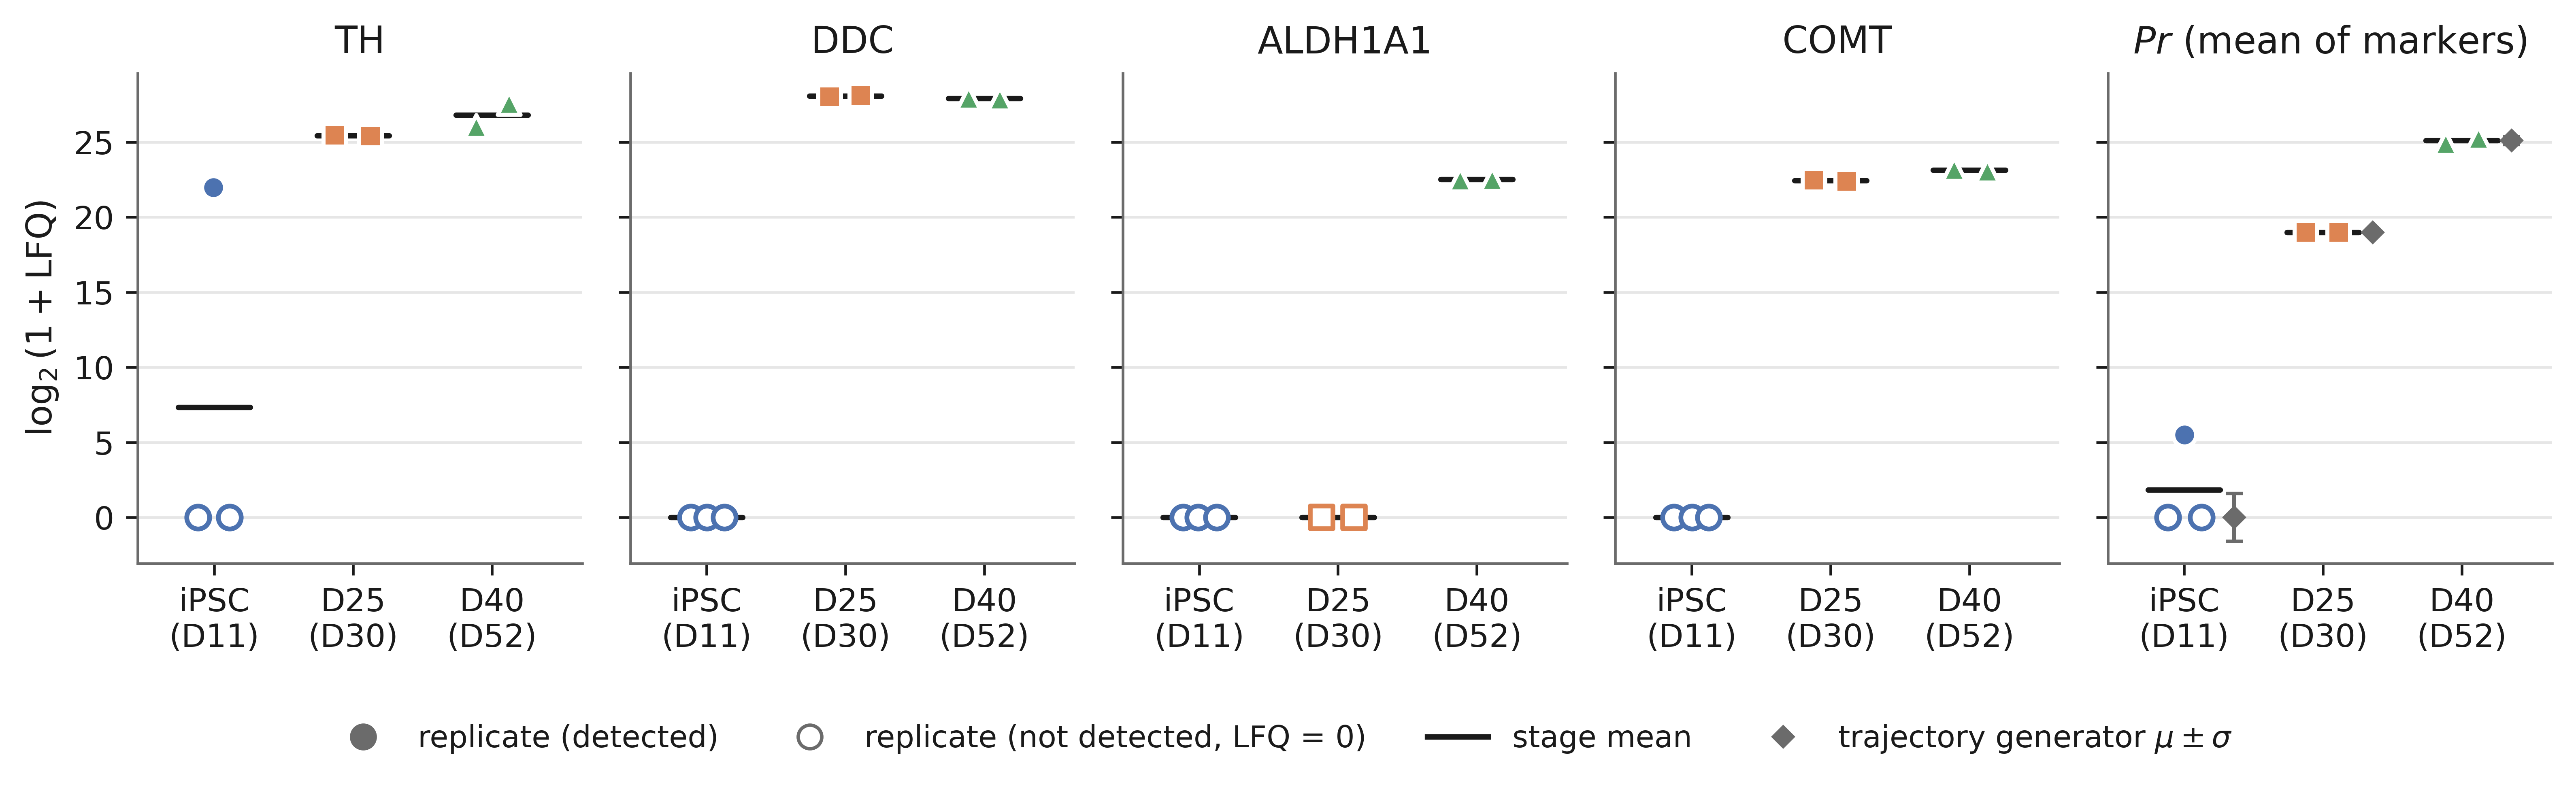
\includegraphics[width=\textwidth]{images/fig_pr_replicates.png}
\caption*{\textcolor{red}{Fig.~2: \textbf{Individual proteomic CTRL replicates at each stage.} Columns show the four $\mathcal{G}_{Pr}$ markers and the replicate-level $Pr$ score on the $\log_{2}(1+\text{LFQ})$ scale. Filled markers are quantified values; hollow markers are non-detections (LFQ $= 0$; in the $Pr$ panel, replicates with none of the four markers detected). Black bars are stage means. In the $Pr$ panel, grey diamonds with error bars show the mean $\pm$ s.d.\ of the distribution from which per-trajectory $Pr$ values are drawn (Section~3.3); at D11 this is the detection-floor anchor $\mathcal{N}(0, \sigma_{\text{D11}}/2)$ rather than the replicate mean. Stage is encoded by both x-position and marker shape. $n = 3/2/2$ replicates.}}
\end{figure}
\begin{revised}
The figure shows that replicate agreement differs sharply by stage: the two D25 replicates (D30 stage) and the two D40 replicates (D52 stage) agree closely, whereas the three iPSC replicates do not --- TH is quantified in only one of them, and no other marker is detected in any of them.
\end{revised}

\point{\loc{Q5, item 1} The Pr-only model achieves the same stage classification performance as the full 3D model, indicating that stage discrimination is mainly driven by the Pr axis. This finding should be clearly acknowledged in the discussion.}

\reply{We agree and now acknowledge it explicitly in the abstract, in the Task~A results (``We state this explicitly: stage discrimination in the 3D model is driven by the $Pr$ axis''), in the validation summary of the Discussion (Section~5.2), and as Limitation~4. The revised passages are reproduced under Reviews~1.8 and~1.10.}

\point{\loc{Q5, item 2} The reduction in overall MAE does not necessarily indicate improved prediction performance in the original transcriptomic dimensions. The authors should interpret this result more carefully in light of the dimension-specific errors.}

\reply{We agree. We added paired bootstrap confidence intervals for the change in the $P$/$D$-only error; all three include zero, so adding $Pr$ neither improves nor degrades the transcriptomic forecasts. The text now explains why the overall MAE falls anyway (the metric averages over dimensions, and the added dimension is forecast with very low error because it is drawn around a fixed stage centre) and warns against reading the lower overall MAE as better transcriptomic prediction. The abstract, the Table~7 caption, and the conclusion state the same.}

\revisedheading{Section~4.3.2}
\begin{revised}
The paired 95\% bootstrap intervals for the change in $\text{MAE}_{PD}$ between 3D and 2D all include zero (Ridge $[-0.0001, 0.0001]$, Random Forest $[-0.0014, 0.0028]$, Transformer $[-0.0019, 0.0021]$). Adding $Pr$ thus neither helps nor hurts the transcriptomic forecasts. The lower overall MAE must not be read as better prediction of the original transcriptomic dimensions: because Eq.~9 averages over dimensions, appending a third dimension that is forecast with very low error lowers the average even when the first two errors are unchanged. It is low largely because $Pr$ at D52 is drawn around a fixed stage centre (Eq.~6), so its forecast is close to that centre.
\end{revised}

\point{\loc{Q6, item 1} The authors should highlight how proteomic information complements the existing transcriptomic state space, particularly the biological relevance of the four selected markers in dopaminergic differentiation.}

\reply{Section~5.1 now explains the complementarity in biological terms: the transcriptomic $D$ score records whether DA-lineage genes are transcribed, whereas $Pr$ records whether the cells have accumulated the enzymes that make and degrade dopamine and whether they have acquired the A9 phenotype lost in Parkinson's disease. The biological role of each marker is given in Section~3.3 (reproduced under Review~2.2).}

\revisedheading{Section~5.1}
\begin{revised}
The central finding is that adding a measured proteomic axis resolves stage ambiguity that the transcriptomic state cannot: the D30 peak of the $D$ score makes D30 and D52 hard to tell apart from transcripts, whereas the DA-pathway proteins keep rising from D25 to D40 (Table~1). The complementarity is biological as well as statistical. The $D$ score records whether DA-lineage \textit{genes} are transcribed, including transcription factors whose expression is transient; $Pr$ records whether the cells have accumulated the \textit{enzymes} that make and degrade dopamine --- TH and DDC for synthesis, COMT for catabolism --- and, through ALDH1A1, whether they have acquired the A9 substantia nigra phenotype lost in Parkinson's disease. Protein abundance can keep rising after transcript levels plateau or fall, so $Pr$ can reflect functional maturation that transcript-based scores do not, consistent with the weak mRNA--protein correlation reported in DA contexts. These are also the proteins through which many dopaminergic drugs act (e.g.\ DDC and COMT inhibitors used in Parkinson's therapy), which is why a protein-level axis is needed for the drug-screening use the framework is ultimately aimed at.
\end{revised}

\point{\loc{Q6, item 2} The Pr-only baseline, permutation tests, and LORO analysis are valuable validation experiments. Their contributions should be summarized more clearly in the discussion.}

\reply{We added Section~5.2, ``What the validation experiments establish'', which summarises each experiment as the question it answers and its result. The full text is reproduced under Review~1.10.}

\point{\loc{Q6, item 3} The practical role of blockchain-based provenance in managing multi-source omics data and verifying data integrity should be explained more explicitly.}

\reply{We explain the practical role in two places: a plain-language description of the verification procedure in Section~3.4 (reproduced under Review~1.11), and a shortened Discussion paragraph that gives the concrete reasons it mattered in this multi-source pipeline.}

\revisedheading{Section~5.5}
\begin{revised}
Most biomedical provenance systems record where data came from but not how they were processed; the layer here records both, the fingerprint of every input file and the code version of every run. Its practical value in this study is concrete: the proteomic input exists in two versions (a local re-processing and the authors' canonical table), the stage mapping changed during the project, and the transcriptomic and proteomic data come from different laboratories. Without a fixed record, a reader could not tell which of these versions produced a published number; with it, any reader can check in milliseconds and at no cost that their files are the ones used. Integrity holds under the permissioned chain's proof-of-authority trust model, so the contribution is verifiable provenance infrastructure, not a security guarantee against an adversarial public network, and it is secondary to the modelling results.
\end{revised}

\point{\loc{Q7, item 1} The transcriptomic and proteomic datasets were obtained from different studies, potentially introducing differences in experimental conditions and batch effects. This should be discussed further.}

\reply{This is now Limitation~2. It names the sources of cross-study difference, explains their possible effect, notes that the model cannot learn a cell-level relation between the modalities because $Pr$ is drawn independently of $P$ and $D$, and identifies paired measurements from the same cultures as the remedy (also added to Future directions).}

\revisedheading{Section~5.6, Limitation~2}
\begin{revised}
\textit{(2) Cross-study integration.} Transcriptomics and proteomics come from different laboratories, cell lines, protocols, and sampling days, so stage-matched values are paired at the population level, not measured in the same cells or the same cultures. Laboratory and batch effects, protocol differences, and the 5--12-day offsets between matched stages (and the iPSC-versus-progenitor mismatch at the first stage) may shift the proteomic values relative to the transcriptomic ones. Because $Pr$ is drawn independently of $P$ and $D$, the model cannot learn any cell-level relation between the modalities, and the within-stage orthogonality is a property of the construction rather than a biological finding. Paired multi-omic measurements from the same cultures would remove this limitation.
\end{revised}

\point{\loc{Q7, item 2} The limited number of biological replicates in the proteomic dataset, particularly at D30 and D52, may affect the stability of the statistical estimates.}

\reply{Addressed in Limitation~1 and in the Task~A results; both are reproduced under Review~1.5, and the effect on the estimates is discussed under Review~2.8. Limitation~1 singles out the D30 standard deviation estimated from two replicates.}

\point{\loc{Q7, item 3} The study lacks external validation using independent datasets, different cell lines, or alternative differentiation protocols. The generalizability of the proposed model therefore remains to be established.}

\reply{We agree and state this as Limitation~3, together with the pseudo-trajectory nature of the trajectories. Validation on independent cell lines and protocols is listed in Future directions.}

\revisedheading{Section~5.6, Limitation~3}
\begin{revised}
\textit{(3) No external validation.} All results come from one scRNA-seq dataset and one proteomic dataset. The framework has not been tested on independent datasets, other iPSC lines, or other DA differentiation protocols, and its generalisability remains to be established. The 200 trajectories are pseudo-trajectories built from independent cells rather than lineage-traced paths, and are fixed across seeds.
\end{revised}

\point{\loc{Q7, item 4} Drug perturbation prediction and virtual screening have not been directly validated experimentally, and their potential applications should be discussed with appropriate caution.}

\reply{We added Limitation~7, rewrote the Future directions paragraph in conditional terms, and qualified the drug-screening statements in the abstract and conclusion.}

\revisedheading{Section~5.6, Limitation~7, and Section~5.7}
\begin{revised}
\textit{(7) Drug-perturbation use is not yet validated.} No drug perturbation was modelled or tested in this study. The applications to perturbation prediction and virtual screening discussed below are prospective; they would require perturbation data for training and experimental validation of predicted responses before any use in drug development.

[\ldots] If such a model were trained on perturbation data and its predictions confirmed experimentally, it could support virtual drug screening for Parkinson's disease: candidate compounds targeting the dopamine synthesis pathway could be ranked by the proximity of their predicted D52 states to a target therapeutic phenotype, to prioritise --- not replace --- wet-lab experiments. None of these steps has been validated yet.
\end{revised}

\point{\loc{Q8, item 1} The objectives and main contributions should be stated more clearly at the end of the Introduction.}

\reply{The Introduction now ends with an Objectives paragraph followed by the contribution list ordered by importance. Both are reproduced under Review~1.1.}

\point{\loc{Q8, item 2} The matching strategy and sample correspondence between the two datasets should be described more systematically in the Methods section.}

\reply{The matching strategy is now a dedicated Methods subsection (Section~3.2.3) with explicit matching rules, a stage-correspondence table (Table~2), and a per-replicate sample table (Table~3). These are reproduced under Reviews~2.3, 2.5, and~2.10.}

\point{\loc{Q8, item 3} The Results section should clearly distinguish stage classification from trajectory prediction to avoid confusion about their respective implications.}

\reply{The benchmark results are now split into two subsections, ``Stage classification (Task~A): a separability check'' (Section~4.3.1) and ``Trajectory prediction (Task~B)'' (Section~4.3.2), introduced by a paragraph that states what each task measures and that a result on one carries no implication for the other.}

\revisedheading{Section~4.3}
\begin{revised}
The two tasks answer different questions and are reported separately. Task~A (stage \textit{classification}, Section~4.3.1) asks whether the stages can be told apart from a single state vector; it characterises the representation. Task~B (trajectory \textit{prediction}, Section~4.3.2) asks how well the late-stage state can be forecast from earlier states; it is the forecasting question a digital twin is built for. A result on one task carries no implication for the other.
\end{revised}

\point{\loc{Q8, item 4} Some technical details regarding blockchain deployment and smart contracts could be shortened or moved to the Supplementary Materials.}

\reply{We moved the compiler settings (Solidity version and EVM options) and six deployment metrics (SHA-256 throughput, per-source latency, gas per transaction, chain ID, bytecode size, and confirmation depth) to the new Supplementary Table~S1, trimmed Table~10 to the verification-relevant metrics, and shortened the blockchain discussion to one paragraph (reproduced under Review~2.16).}

\revisedheading{Supplementary Table~S1 (new)}
\begin{table}[!htbp]
\centering
\caption{\textcolor{red}{Supplementary Table~S1. PureChain deployment and performance metrics moved from the main text.}}
\color{red}
\begin{tabular}{ll}
\toprule
Metric & Value \\
\midrule
Contract address & \texttt{0xFA954E93c389D54B05FBA832276B7C7a42bAeD51} \\
Chain ID & 900520900520 \\
Compiler & Solidity 0.8.20 (\texttt{evmVersion: paris}, \texttt{viaIR: true}) \\
Contract bytecode & 4,716 bytes \\
SHA-256 throughput & 298\,MB/s \\
Per-source registration latency (Novak) & 33\,ms \\
Per-transaction gas (Jerber / Novak) & 405,683 / 472,168 \\
Per-transaction cost & 0\,PCG (gas-free) \\
Confirmation depth & 72,011 blocks since registration \\
\bottomrule
\end{tabular}
\end{table}

\point{\loc{Q9} Could the manuscript benefit from language editing? Yes.}

\reply{Please see our reply to Review~1.15: the complete manuscript was proofread, all new and rewritten passages were edited for clarity and concision, terminology was standardised, and the abstract was rewritten in full. Language-only corrections are shown in red without a superscript tag.}

\section*{Closing Statement}
We again thank the Associate Editor and both reviewers for comments that materially improved the paper. The revision now states a single primary objective and keeps stage separability and trajectory prediction apart; documents the proteomic processing, the cross-study stage correspondence, and every replicate used; describes trajectory and $Pr$ construction exactly as implemented, including the corrections listed above; reports confidence intervals and the dimension-specific source of the Task~B gain; and states the limitations of a 3/2/2-replicate, cross-study design without overstating what the perfect separability or the MAE reduction show.

\end{document}
